%----------------------------------------------------------------------------
\chapter{Első fázis}\label{sect:FirstPhase}
%----------------------------------------------------------------------------
\section{Szöveges UseCase(k)}
\subsection{Main Scenerio}
\begin{enumerate}
	\item Bejelentkezés
		\begin{itemize}
			\item Elsődleges aktor: vizsgálatot végző munkatárs
			\item Elsődleges, sikeres forgatókönyv: A vizsgálatot végző munkatárs megadja az azonosítóját és jelszavát.
		\end{itemize}	
	\item A rendszer megjeleníti a főmenüt
	\item Az alkoholszondás vizsgálathoz tartozó jegyzőkönyvsablon kiválasztása
		\begin{itemize}
			\item Elsődleges aktor: vizsgálatot végző munkatárs
			\item Elsődleges, sikeres forgatókönyv: A vizsgálatot végző munkatárs kiválasztja az alkoholszondás vizsgálat jegyzőkönyv sablont.
		\end{itemize}
	\item A rendszer elküldi a megfelelő sablont
	\item Jegyzőkönyv felvétele
		\begin{itemize}
			\item Elsődleges aktor: vizsgálatot végző munkatárs
			\item Elsődleges, sikeres forgatókönyv: A vizsgálatot végző munkatárs felveszi a vizsgált munkatárs nevét és azonosítóját, illetve a vizsgálatot kérő felettes nevét és azonosítóját, ezeken felül meg kell adnia még a saját nevét és azonosítóját. A jegyzőkönyvben rögzítenie kell továbbá a vizsgálat eredményét, illetve a vizsgált munkatárs megjegyzését. 
		\end{itemize}
	\item A rendszer megerősíti a kitöltött adatok hitelességét
	\item Jegyzőkönyv aláírása
	\begin{itemize}
		\item Elsődleges aktor: az eljárásban résztvevő személy 
		\item Elsődleges, sikeres forgatókönyv: Az eljárásban résztvevő személy aláírja a jegyzőkönyvet.
	\end{itemize}
	\item A rendszer jóváhagyja, hogy a megfelelő személyek aláírták a jegyzőkönyvet
	\item A rendszer feltölti a szerverre az elkészített jegyzőkönyvet
	\item A rendszer üzenetet küld, a sikeres jegyzőkönyv felvételéről
\end{enumerate}

\subsection{Extensions}
\begin{description}
	\item [7/a] Vérvizsgálat opcionális igénylése
		\begin{itemize}
			\item Elsődleges aktor: vizsgálatot végző munkatárs
			\item Alternatív forgatókönyv: Abban az eseten ha a szondás vizsgálat eredményével nem ért egyet a vizsgált munkatárs, vérvizsgálatot kér. A \textbf{8/a} UseCase következik ez után.
		\end{itemize}
	\item [8/a] Vérvizsgálati eredmény csatolása
		\begin{itemize}
			\item Elsődleges aktor: üzemorvos
			\item Alternatív forgatókönyv:  Az üzemorvos tetszőleges jegyzőkönyvhöz mellékletet is csatolhat, természetesen ennek csak akkor van értelme ha a vizsgált munkatárs vérvizsgálatot kér. Minden esetben amikor csatol az üzemorvos valamit egy jegyzőkönyvhöz alá is kell írnia azt, így a \textbf{9/a} UseCase következik.
		\end{itemize}
	\item [9/a] A rendszer ellenőrzi az üzemorvos által csatolt fájl hitelességét. Helyes csatolás esetén a \textbf{7-es} UseCase következik, ellenkező esetben visszaugrik a \textbf{8/a}-ra.
	%\hrule
	%-----------------------------------------------------
	%TODO átírni az összes szart!!!!!
	%-------------------------------------------------
	\item [2/a] Nem megfelelő bejelentkezési adatok. Ugrás az \textbf{1-es} UseCase-re.
	\item [6/a] A rendszer hibát talált az adatok kitöltésénél. 5-ös UseCase következik.
	\item [9/b] Hiányzó vagy hibás aláírás esetén a 7-es UseCase következik.
	\item [9/c] A rendszer hibát talált a fájl csatolásánál. 6-os UseCase következik.
\end{description}

\newpage
\section{Aktivitás diagram}

\begin{figure}[!h]
	\centering
	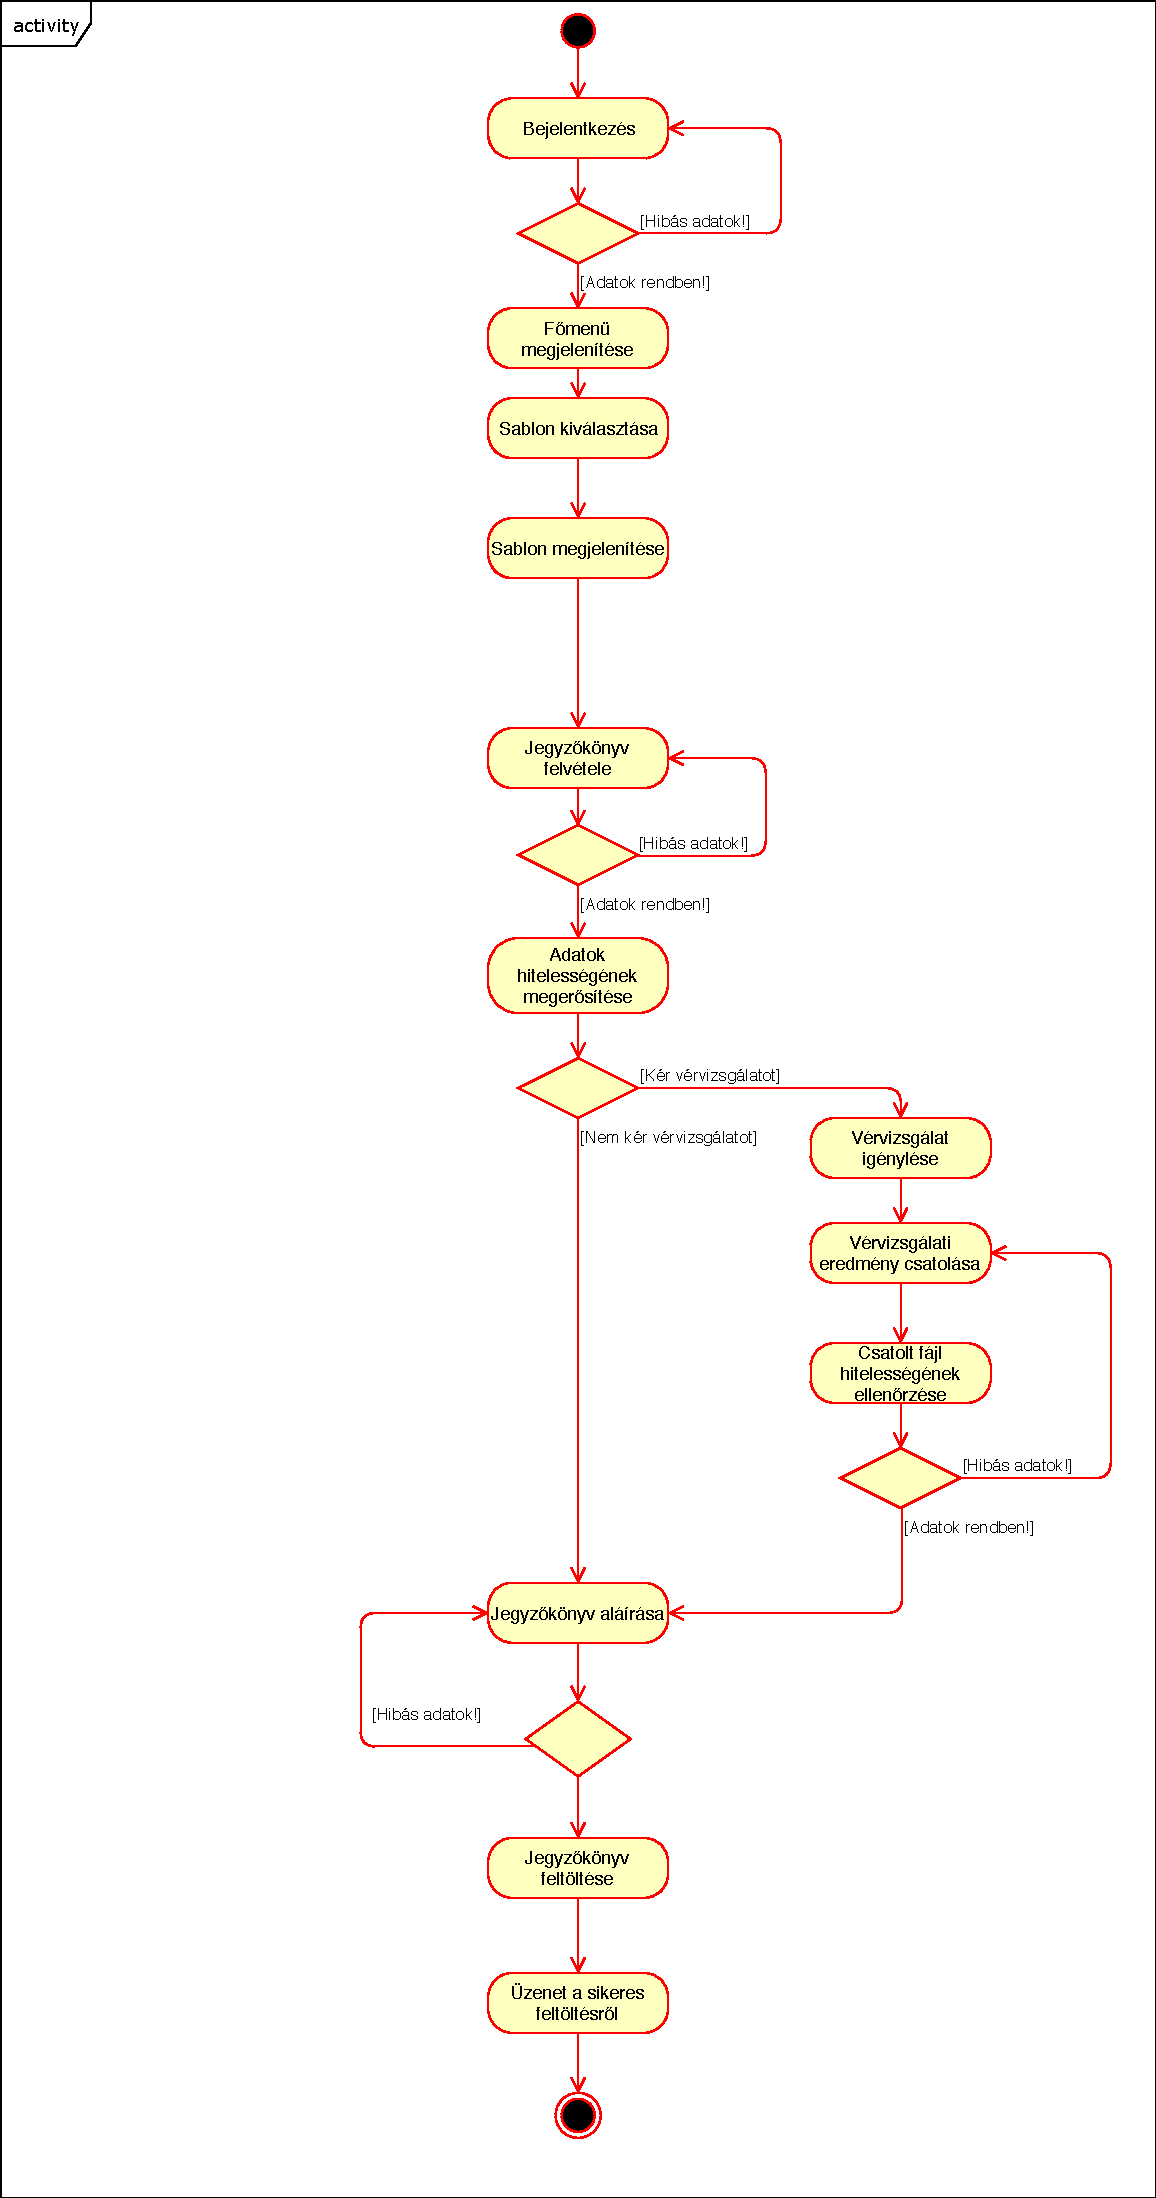
\includegraphics[width=120mm, keepaspectratio]{figures/activity.pdf}
	%\caption{Az aktivitás diagram} 
	%\label{fig:SpiFig}
\end{figure}
\newpage
\section{System sequence diagram}

\begin{figure}[!h]
	\centering
	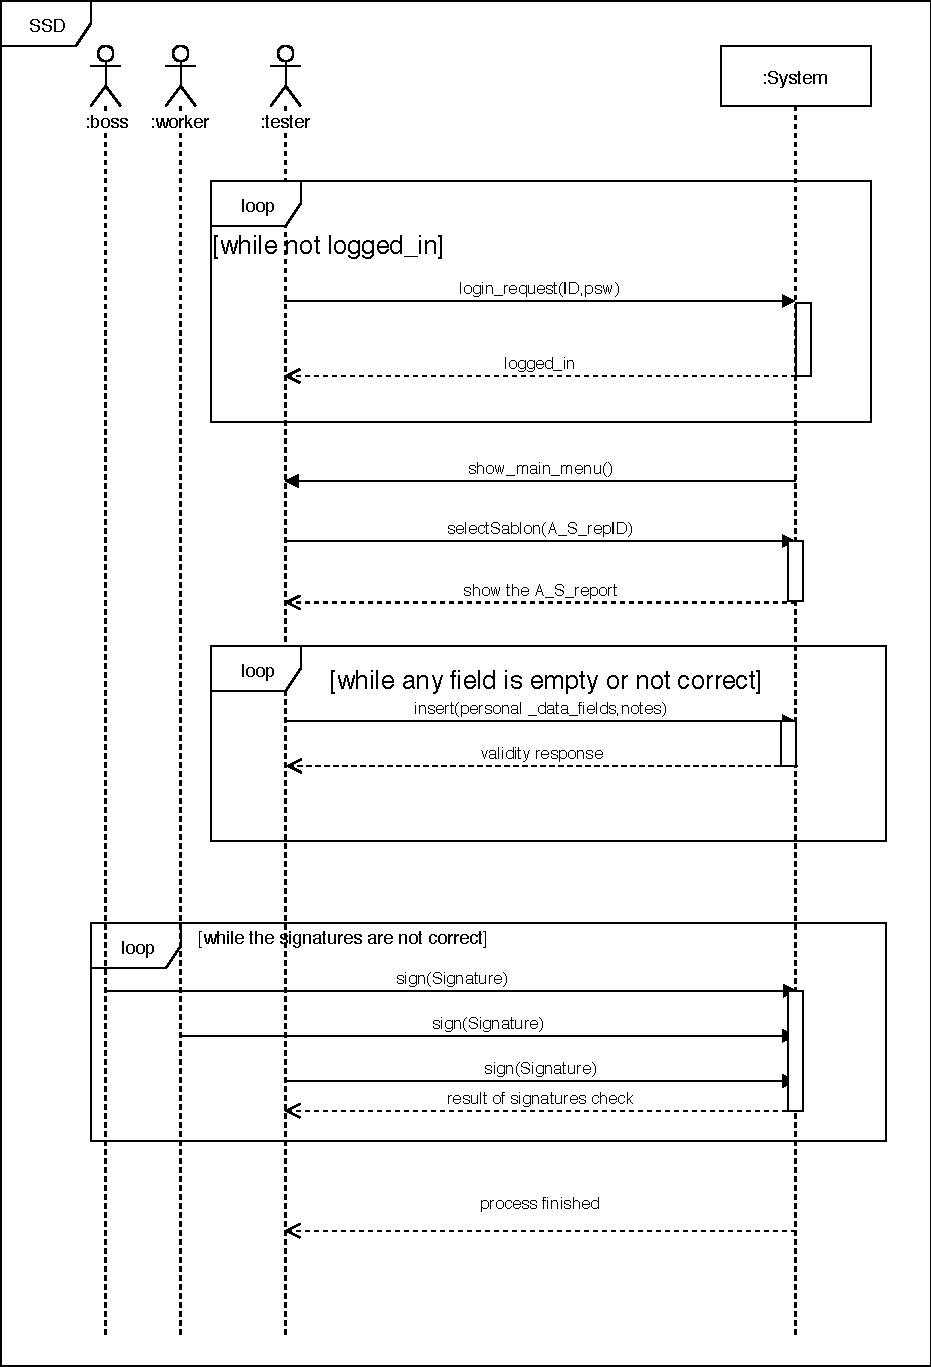
\includegraphics[width=120mm, keepaspectratio]{figures/ssd.pdf}
	%\caption{Az aktivitás diagram} 
	%\label{fig:SpiFig}
\end{figure}

\begin{figure}[!h]
\centering
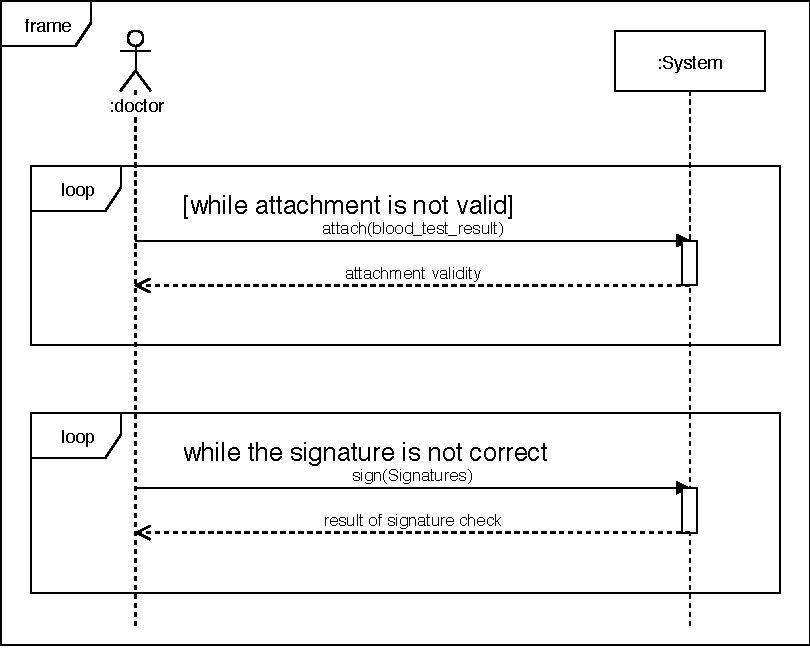
\includegraphics[width=120mm, keepaspectratio]{figures/ssd2.pdf}
%\caption{Az aktivitás diagram} 
%\label{fig:SpiFig}
\end{figure}
